\documentclass[pdf,bluish,slideColor,colorBG]{prosper}
\hypersetup{pdfpagemode=FullScreen}
\usepackage{color}
\usepackage{graphicx}
\usepackage{amsfonts}
\usepackage{amsmath}
\usepackage{hyperref}
\def\baselinestretch{0.7}
\parindent 0.3in
\hyphenpenalty=10000
\tolerance=10000
\pagestyle{empty}

\def\Prob{{\rm Prob\;}}
\def\prob{{\rm \;Prob\;}}
\def\Var{{\rm Var}}        % Var
\def\Cov{{\rm Cov}}        % Cov

\DeclareSymbolFont{AMSb}{U}{msb}{m}{n}
\DeclareMathSymbol{\expect}{\mathalpha}{AMSb}{'105}

% bold math (use \bm{...})
\def\bm#1{\mathpalette\bmstyle{#1}}
\def\bmstyle#1#2{\mbox{\boldmath$#1#2$}}

\title{Quantitative genetics: Variance components and heritability}

\author{Joe Felsenstein}

\institution{11 October 2016}

\subtitle{Bio 550D: Morphometrics in Biology}


\definecolor{orange}{rgb}{1.0,0.8,0.0}
\definecolor{Dandelion}{rgb}{0.8,0.4,0.3}
\definecolor{golden}{rgb}{1.0,0.75,0.2}
%\definecolor{golden}{rgb}{1.0,0.8,0.3}
\definecolor{purple}{rgb}{0.6,0.2,0.6}
\definecolor{darkblue}{rgb}{0.1,0.1,0.6}
\definecolor{yellow}{rgb}{1.0,1.0,0.0}
\definecolor{brightred}{rgb}{1.0,0.,0.0}
\definecolor{black}{rgb}{0.0,0.0,0.0}
\definecolor{white}{rgb}{1.0,1.0,1.0}
\definecolor{purple}{rgb}{0.8,0.0,0.8}

% sets backgroundcolor for whole document 
%\pagecolor{darkblue}
%\pagecolor{white}
% sets text color
%\color{yellow}
%\color{black}
% to change just a few words
% using \textcolor{color}{text}

\DeclareSymbolFont{AMSb}{U}{msb}{m}{n}
\DeclareMathSymbol{\expect}{\mathalpha}{AMSb}{'105}

\def\Prob{{\rm Prob\;}}
\def\prob{{\rm \;Prob\;}}
\def\Var{{\rm Var}}        % Var
\def\Cov{{\rm Cov}}        % Cov

\begin{document}

% OUTLINE ALL TALKS
% Brownian motion approximation
% Edwards and Cavalli-Sforza
% me, 1968/1973
% Lande, 1976 
% REML trees with Brownian motion
% Pruning
% Inferring the covariances?
% incl. Grafen (and/or PGLS)
% The determinant result (make sure Jacobian included)
% Some kind of simulation with finite number of loci w/mutation
% 
% Source of covariation (VA, selective)
% 
% Ornstein-Uhlenbeck (Marguerite?)
% Chasing a peak
% Go where peak goes
% Smoothing caused by this
% Equilibrium covariances
% Tree covariation
% 
% Morphometrics
% Bookstein
% Alignment
% Rotation and optimization (and approximations)
% Need for special models

% Threshold models
% Sewall Wright( and guinea pig)
% 


\maketitle

{\parindent=0in


\begin{slide}[Replace]{Development of quantitative genetics theory}
\bigskip

\begin{center}
\begin{tabular}{c  c c c}
\includegraphics[width=0.8in]{galton.ps} &
\includegraphics[width=0.75in]{pearson.ps} &
\includegraphics[width=0.75in]{Fisher.ps} &
\includegraphics[width=0.8in]{Lush.ps}\\
\multicolumn{2}{c}{\parbox[t]{1.5in}{
\begin{flushleft}
Empirical statistical models
(their ``Law of Ancestral Heredity'')
by Galton and Pearson from 1889 on ...
\end{flushleft}}
}
&
\parbox[t]{1.0in}{
\begin{flushleft}
... were overwhelmed by
R. A. Fisher's 1918
Mendelian tour-de-force
\end{flushleft}}
&
\parbox[t]{1.0in}{
\begin{flushleft}
... which Jay Lush and his
colleagues made the center of
modern animal and plant breeding
\end{flushleft}}
\end{tabular}
\end{center}

\end{slide}

\begin{slide}[Replace]{We use the standard quantitative genetic model}

\centerline{\includegraphics[height=2.8in]{quantmodel1.idraw}}

\end{slide}

\begin{slide}[Replace]{We use the standard quantitative genetic model}

\centerline{\includegraphics[height=2.8in]{quantmodel2.idraw}}

\end{slide}

\begin{slide}[Replace]{We use the standard quantitative genetic model}

\centerline{\includegraphics[height=2.8in]{quantmodel3.idraw}}

\end{slide}

\begin{slide}[Replace]{We use the standard quantitative genetic model}

\centerline{\includegraphics[height=2.8in]{quantmodel4.idraw}}

\end{slide}

\begin{slide}[Replace]{We use the standard quantitative genetic model}

\centerline{\includegraphics[height=2.8in]{quantmodel5.idraw}}

\end{slide}

\begin{slide}[Replace]{ ... which leads to various character values}

\centerline{\includegraphics[height=2.8in]{quantmodel6.idraw}}

\end{slide}

\begin{slide}[Replace]{ ... which leads to various character values}

\centerline{\includegraphics[height=2.8in]{quantmodel7.idraw}}

\end{slide}

\begin{slide}[Replace]{ ... which leads to various character values}

\centerline{\includegraphics[height=2.8in]{quantmodel8.idraw}}

\end{slide}

\begin{slide}[Replace]{ ... which leads to various character values}

\centerline{\includegraphics[height=2.8in]{quantmodel9.idraw}}

\end{slide}

\begin{slide}[Replace]{ ... which leads to various character values}

\centerline{\includegraphics[height=2.8in]{quantmodel10.idraw}}

\end{slide}

\begin{slide}[Replace]{ ... to make a 0/1 character apply a threshold of 9}

\centerline{\includegraphics[height=2.8in]{quantmodel12.idraw}}

(This is Sewall Wright's threshold model, a polygenic model of discrete
characters).

\end{slide}

\begin{slide}[Replace]{A single mendelian locus with environmental effects}

\centerline{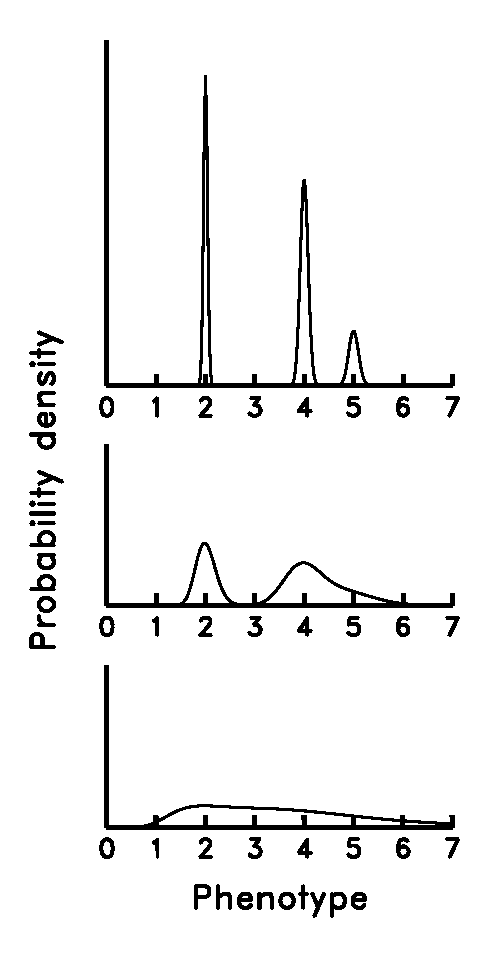
\includegraphics[height=2.4in]{fig9-1.eps}}
\bigskip

In this simulation, each genotype has background environmental variance distributed in a lognormal
distribution.  Those environmental variables get larger as we move from the
top figure downwards.

\end{slide}

\begin{slide}[Replace]{Many mendelian loci and environmental effects}

\begin{center}
\begin{tabular}{c c}
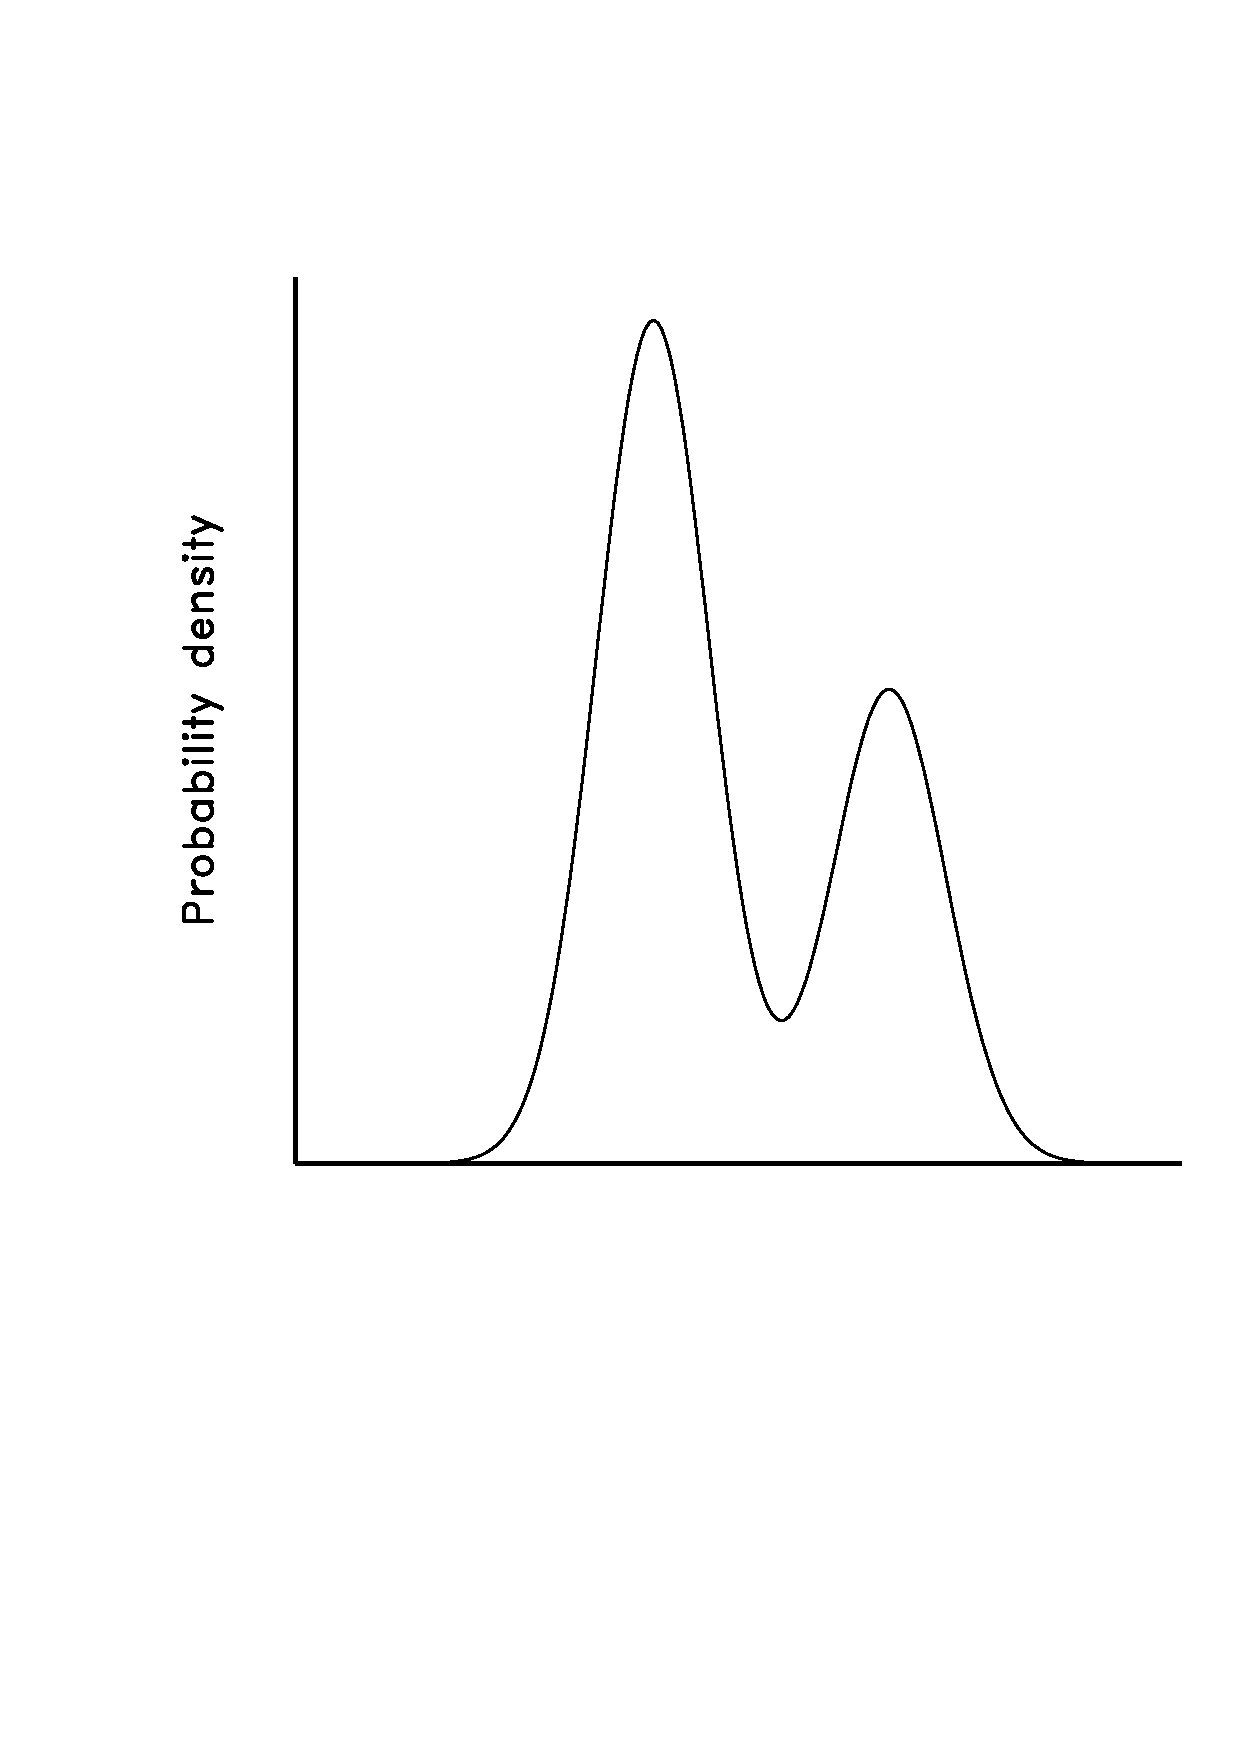
\includegraphics[width=1.15in]{fig9-7a.idraw} &
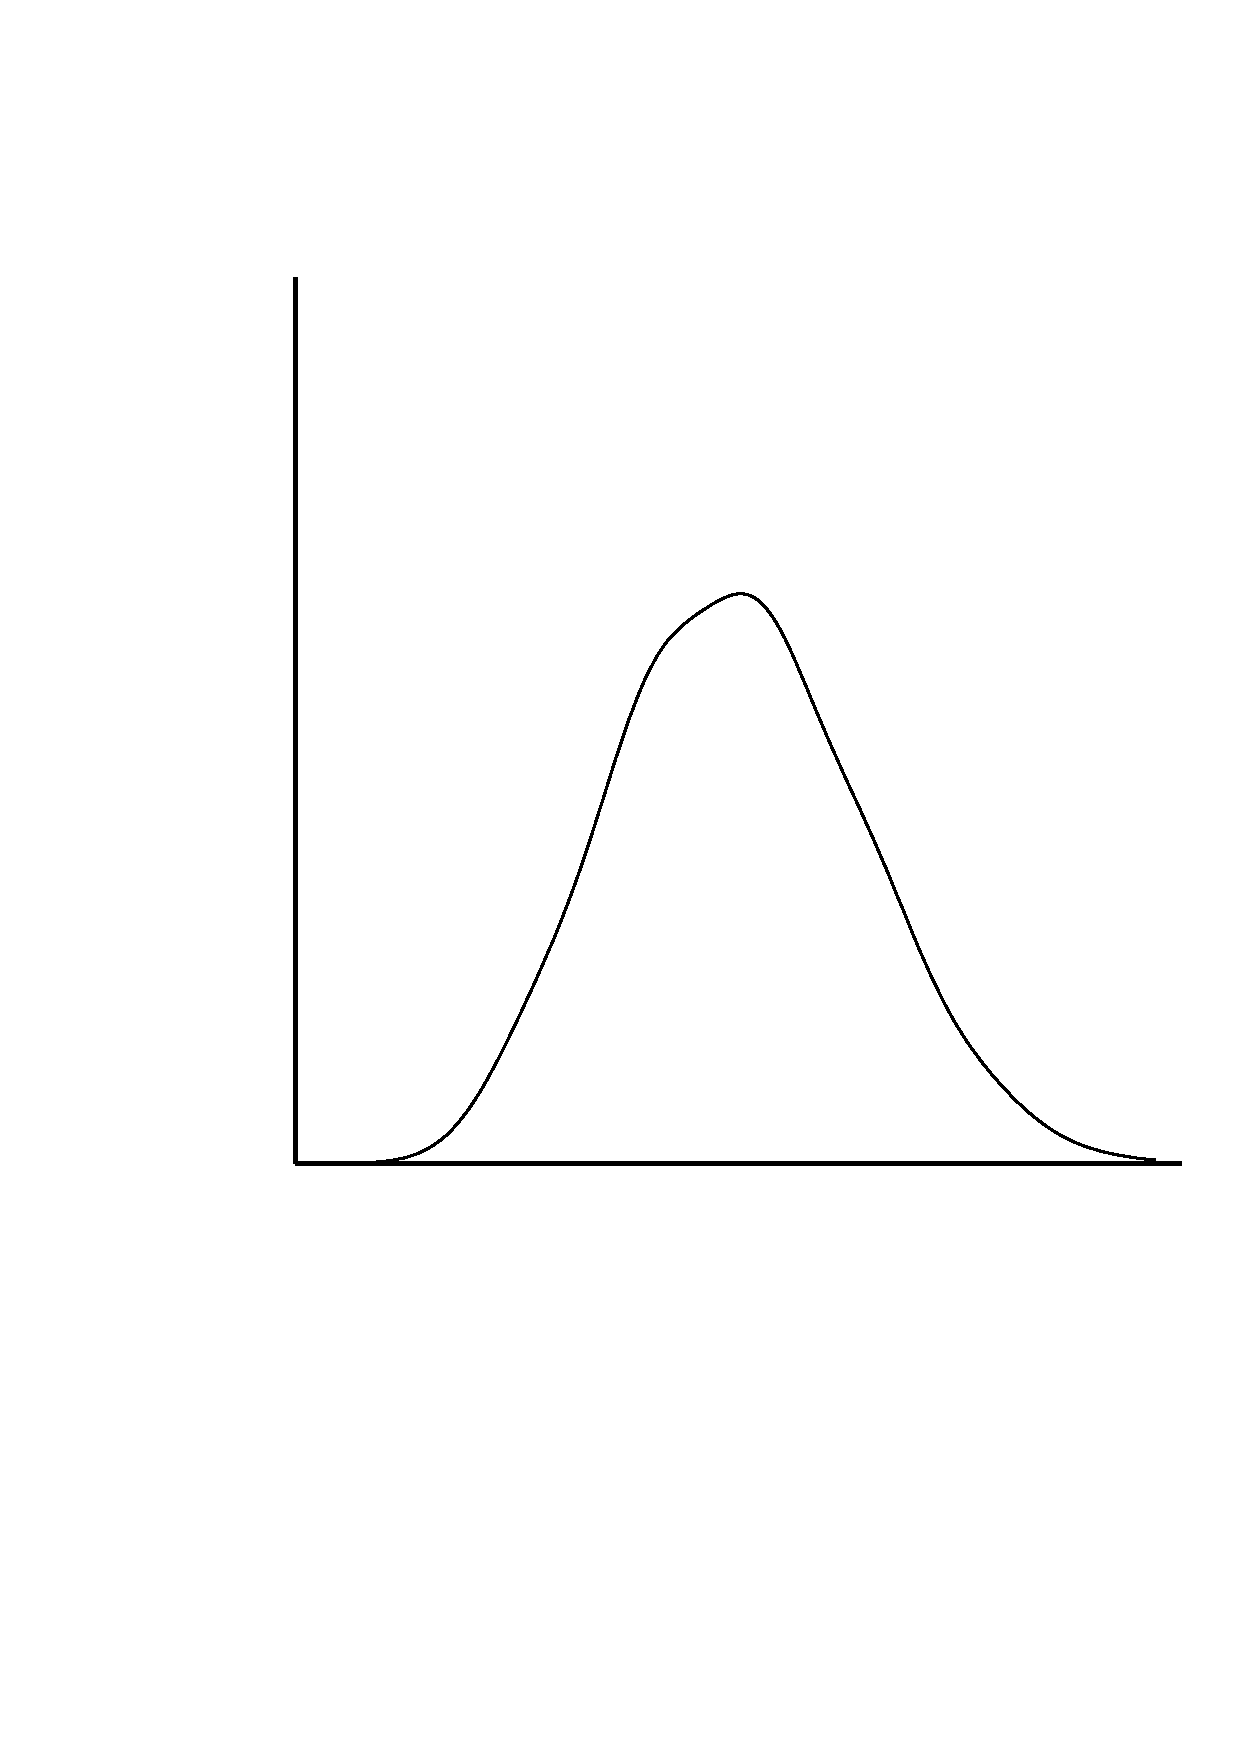
\includegraphics[width=1.15in]{fig9-7c.idraw} \\
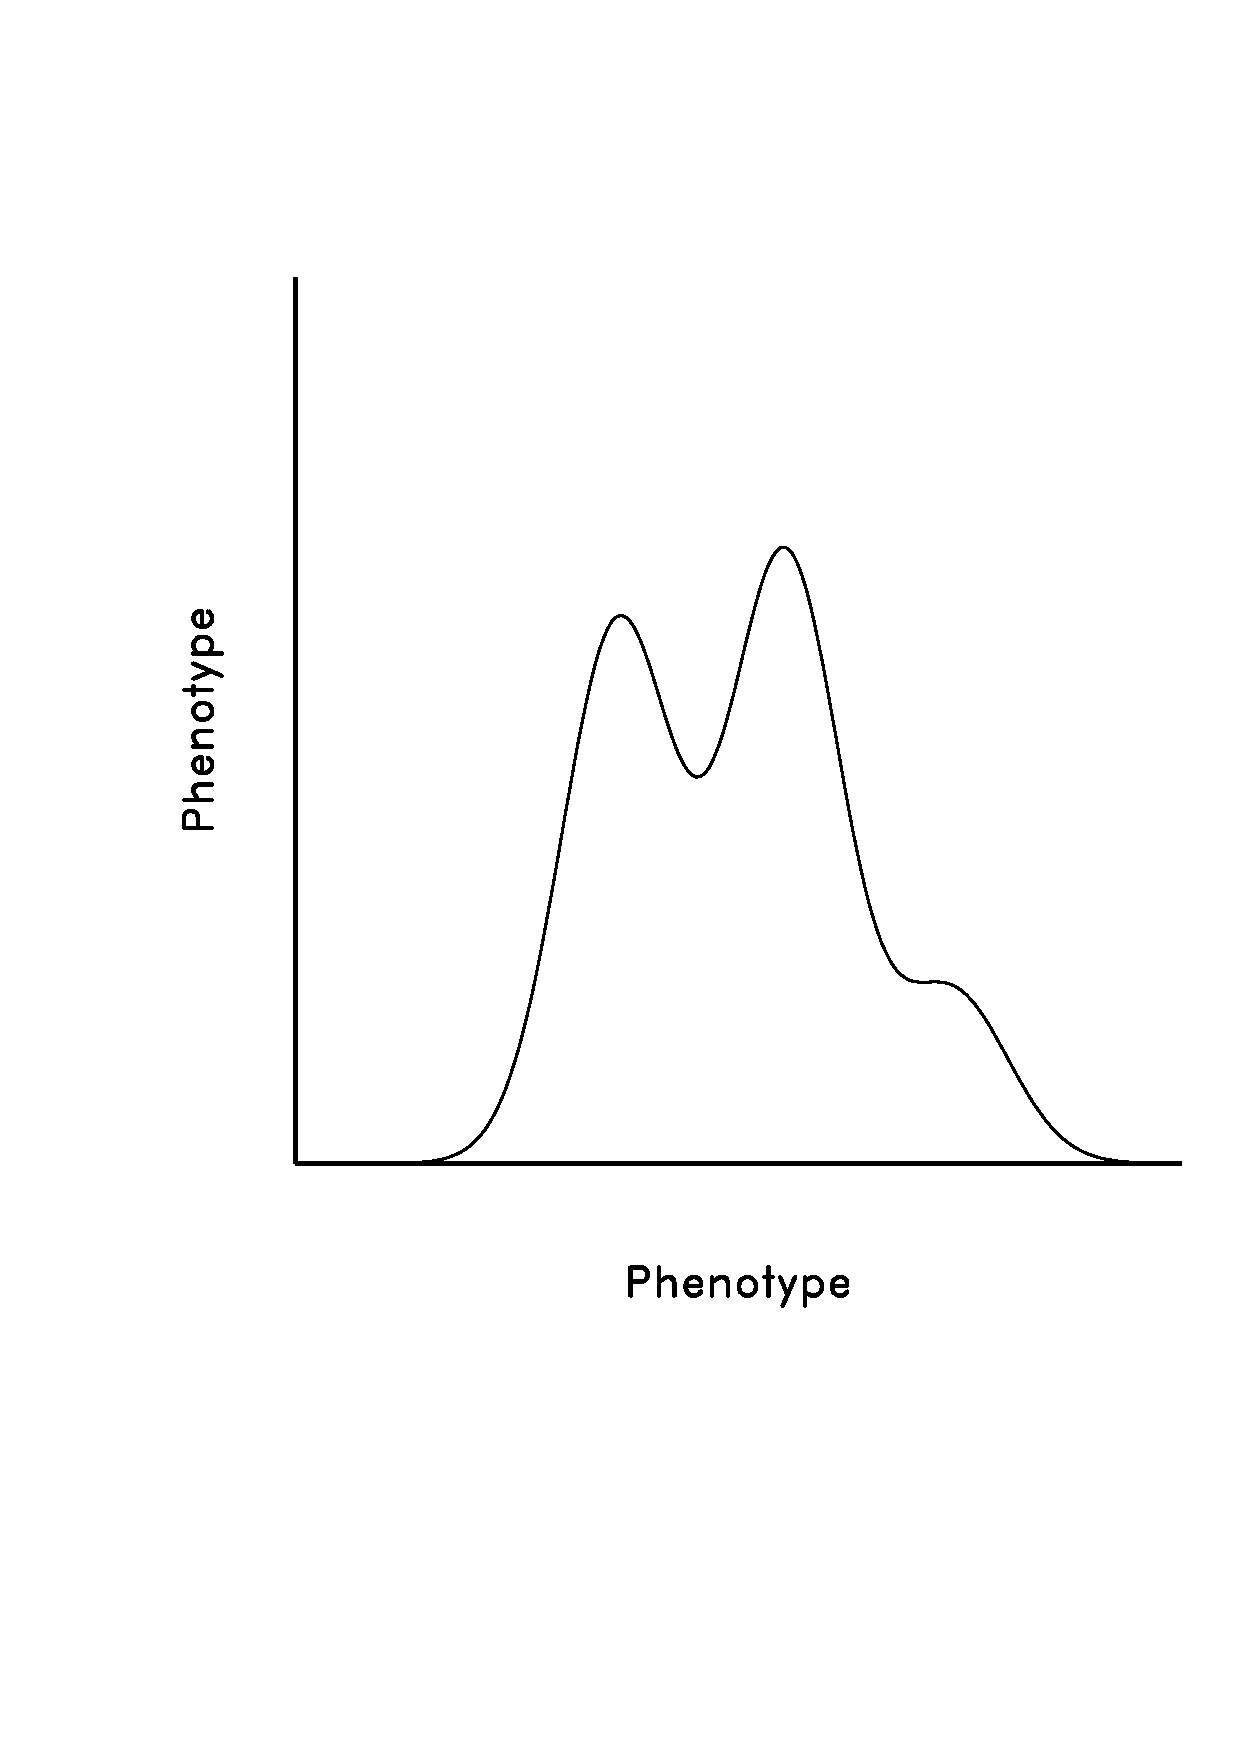
\includegraphics[width=1.15in]{fig9-7b.idraw} &
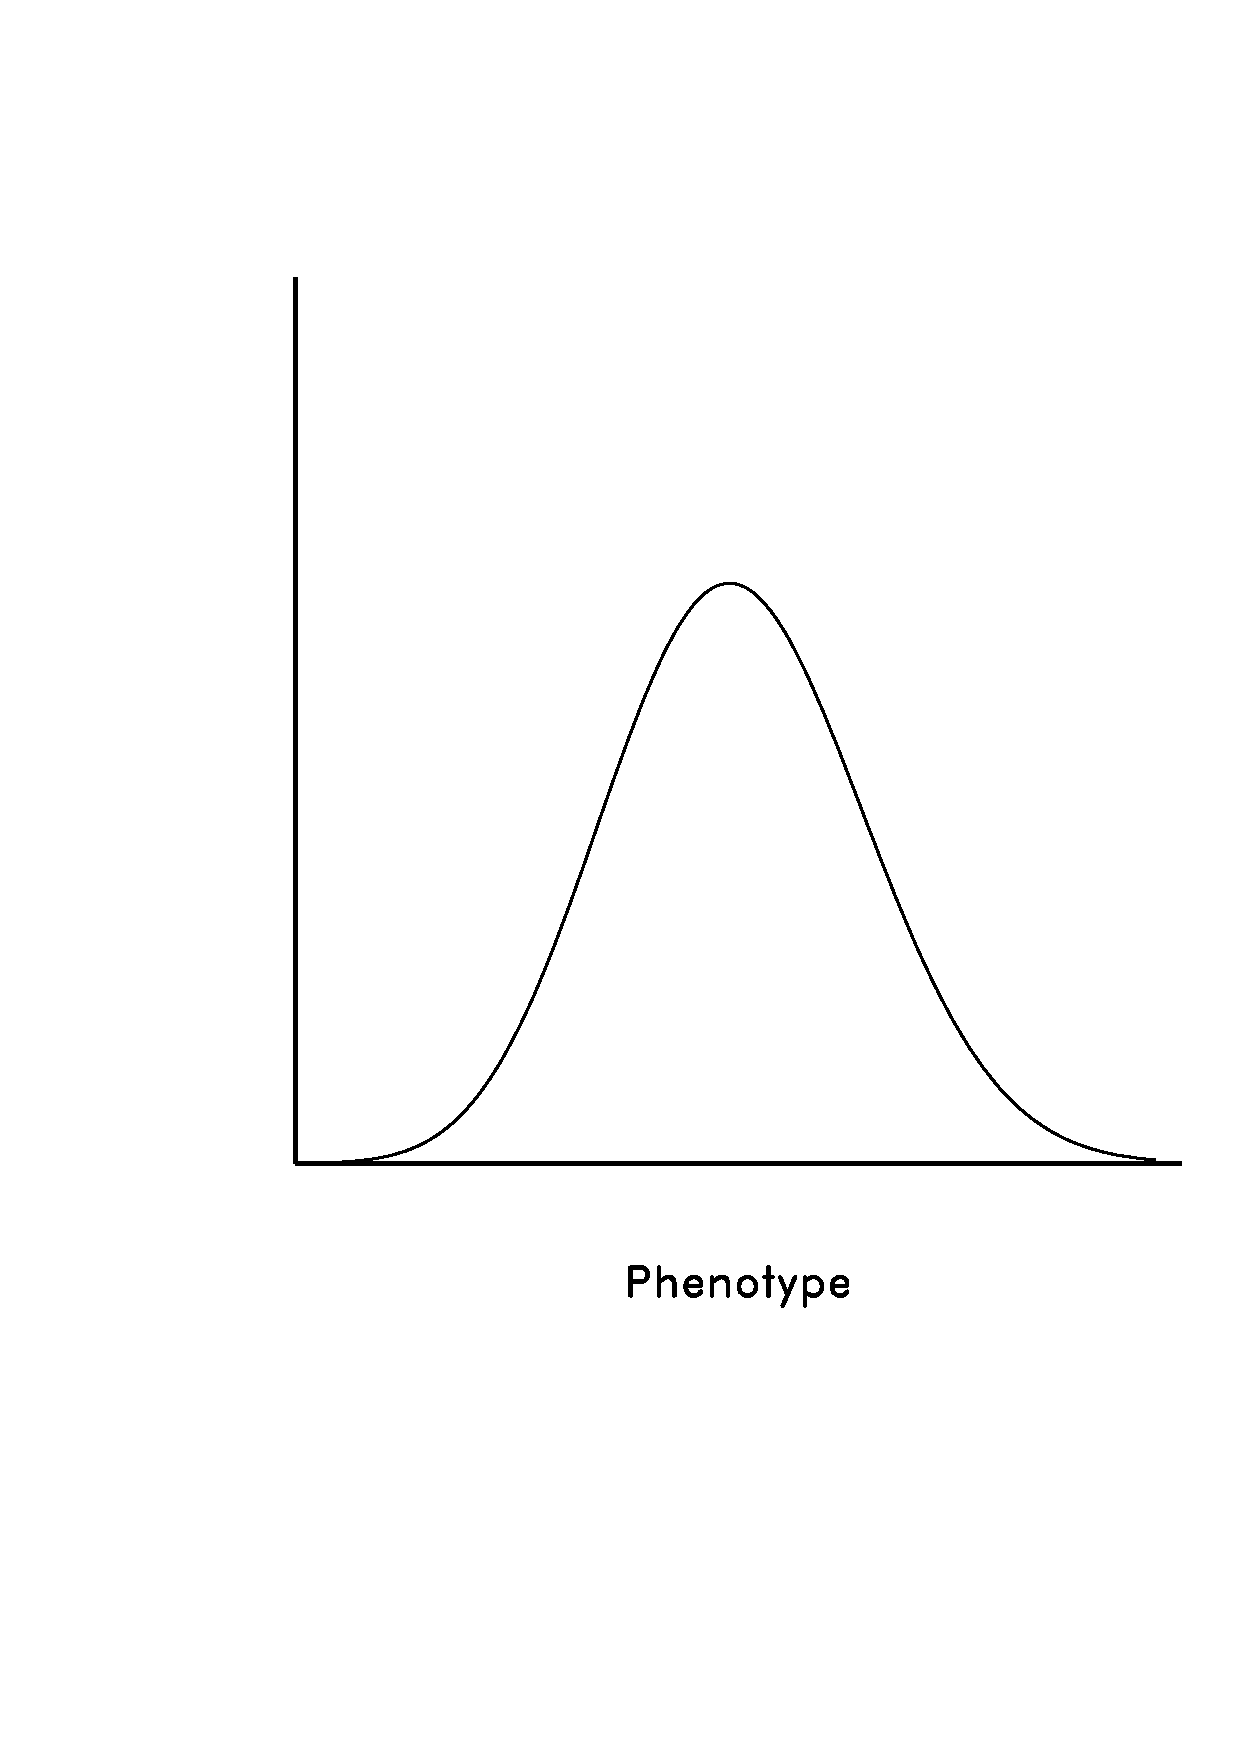
\includegraphics[width=1.15in]{fig9-7d.idraw}
\end{tabular}
\end{center}

(Each locus is dominant and all have the same effect and same gene frequency,
but with the effect sizes scaled in each case to have the same total genetic
variance and to have 30\% of the phenotypic 
variance be genetic).

\end{slide}

\begin{slide}[Replace]{A two-locus model with some interaction between loci}

\begin{tabular}{c c}
{
\parbox[b]{2in}{
\begin{tabular}{c | c c c}
\multicolumn{4}{c}{Means of the genotypes}\\
\renewcommand{\arraystretch}{1.3}
& & & \\
\hline
       &  {\it BB}   &      {\it Bb}   &      {\it bb}\\
\hline
{\it AA}  &    6.5    &     6     &    4\\
{\it Aa}  &    5.5    &     5     &    3.5\\
{\it aa}   &   4.5    &     3    &     2
\end{tabular}
\vspace{0.9in}

\begin{flushleft}
Greater (lognormal) environmental variance
as one moves from the top figure to the 
bottom.
\end{flushleft}
}}
& 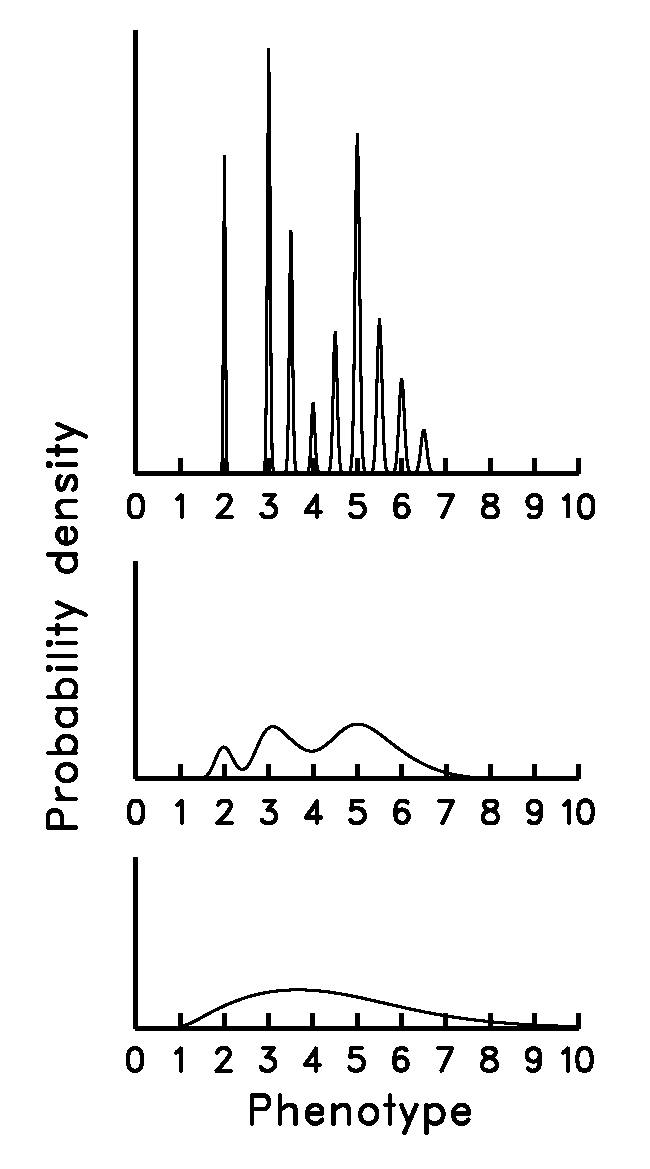
\includegraphics[height=2.4in]{fig9-2.eps}
\end{tabular}
\end{slide}

\begin{slide}[Replace]{Additive effects and dominance deviations}

\centerline{\includegraphics[height=2.5in]{fig9-3.ps}}
\medskip

R. A. Fisher (1918) defined additive effects $\alpha_i$ and dominance
deviations $\delta_{ij}$ by fitting a straight line through the
genotypic mean phenotypes, with points weighted by their Hardy-Weinberg 
population frequency.

\end{slide}

\overlays{5}{
\begin{slide}[Replace]{Fisher's regression partitions the variance}

Fisher's model assumes
\begin{itemstep}
\item Random mating, so Hardy-Weinberg proportions
\item Linkage equilibrium between all loci
\item Environmental effects independent of the genotype
\item Environmental effects independent in different individuals
\item No interaction between loci (effects are additive between loci)
\end{itemstep}

\end{slide}
}

\overlays{4}{
\begin{slide}[Replace]{So the following are uncorrelated in the
population}

\begin{itemstep}
\item The two $\alpha$'s in a locus (by Hardy-Weinberg)
\item The $\alpha$'s and the $\delta$ in a locus, as a result of having defined
them by the weighted least squares regression (trust me)
\item All the effects ($\alpha$'s and $\delta$'s) at different loci (by
linkage equilibrium)
\item The environmental effect (by independence of the environment from the
genotype)
\end{itemstep}

\fromSlide{4}{So the phenotype is a sum of terms, all of which are uncorrelated (have zero
covariance):
\[
\begin{array}{c c l}
\mathsf{P} & \mathsf{=} & \mathsf{\mu \ + \ \alpha^{(1)}_i + \alpha^{(1)}_j + \delta^{(1)}_{ij} \ + \ \alpha^{(2)}_k + \alpha^{(2)}_\ell \ + \delta^{(2)}_{k\ell}}\\
& & \\
& & \mathsf{\ + \ \alpha^{(3)}_m + \alpha^{(3)}_n + \delta^{(3)}_{mn} \ + \ \dots \ + \ \epsilon}
\end{array}
\]
}

\end{slide}
}

\begin{slide}[Replace]{Rearranging and adding up variances}
\bigskip

\[
\begin{array}{c c l}
\mathsf{P} & \mathsf{=} &  \mathsf{\mu \ + \ \left(\alpha^{(1)} + \alpha^{(1)}
\ + \ \alpha^{(2)} + \alpha^{(2)}  +  \alpha^{(3)} + \alpha^{(3)} + \dots \right)}\\
& & \\
& & \mathsf{\ + \ \left( \delta^{(1)} \ + \delta^{(2)} \ + \ \delta^{(3)}\right) \ + \ \dots \ + \ \epsilon}
\end{array}
\]

\noindent
Since random variables that are uncorrelated have variances that sum up,
we have partitioned the phenotype into four uncorrelated parts (one a nonvarying
starting point $\mathsf{\mu}$), 
\[
\mathsf{P \ = \ \mu + A + D + E}
\]

\noindent
The total ``breeding value'' $\mathsf{~A~}$ and the total of the dominance
deviations $\mathsf{D~}$ each have a variance ($\mathsf{V_A}$ and
$\mathsf{V_D}$).  
and those being uncorrelated means that their variances add up too:
\[
\mathsf{\Var(P) \ = \ V_A \ + \ V_D \ + \ V_E}
\]

\end{slide}

\begin{slide}[Replace]{Covariances and fraction of shared effects}
\bigskip

If $\mathsf{X}$, $\mathsf{Y}$, and $\mathsf{Z}$ are independent random variables,
\[
\Cov[X+Y,\ \ X+Z] \ = \ \Var(X)
\]
So the covariance is the variance of the part shared between the two sums.
\[
\begin{array}{c c c c c l}
\mathsf{P_x} & \mathsf{=} &  \mathsf{\mu} \ & \ \mathsf{+ \ (\alpha + \alpha + \alpha + \alpha + \dots\ )} & \mathsf{+ (\delta + \delta + \delta + \dots\ )} & \mathsf{+ \ \ \varepsilon} \\
& & & \uparrow & \uparrow & \\
& & & \mathsf{f_1} {\rm ~of~these~shared~} &  \mathsf{f_2} {\rm ~of~these~shared~} & \\
& & & \downarrow & \downarrow  & \\
\mathsf{P_y} & \mathsf{=} &  \mathsf{\mu} \ & \mathsf{+ \ (\alpha + \alpha + \alpha + \alpha + \dots\ )} & \mathsf{ + (\delta + \delta + \delta + \dots\ )} & \mathsf{ + \ \ \varepsilon}
\end{array}
\]

If a fraction $\mathsf{f_1}$ of the $\mathsf{\alpha}$ are shared, that fraction
of the variance from them is shared, and similarly for the $\mathsf{\delta}$s,
and environment is not shared,
\noindent
\[
\mathsf{\Cov\left(P_x, P_y\right) \ = \ f_1\,V_A \ + \ f_2\,V_D}
\]

\end{slide}

\begin{slide}[Replace]{Variance components and ANOVA}
\bigskip

Does all this look a lot like analysis of variance (ANOVA)?
\medskip

It ought to: that was also developed by R. A. Fisher in the same era, and
published in the early 1920s, very soon after his 1918 paper.

\begin{itemize}
\item Each additive effect is a single-factor (``row'' or ``column'') effects
\item The dominance deviations are two-way interaction effects
\item All interaction effects between loci, and between the environment
and anything else, have been forced to be zero by the assumed model
\item The least squares regression is the same one used to assign fixed
effects in ANOVA
\end{itemize}

\end{slide}

\begin{slide}[Replace]{Variance components and covariances of relatives}
\medskip

This can be done be computing, from the kind of relationship:

\begin{itemize}
\item  the probability that a single copy of a gene is also found in the
relative, as a result of identity by descent ($\mathsf{f_1}$)
\item the probability that both copies at a locus are each found in the relative
($\mathsf{f_2}$)
\end{itemize}

These give the fraction of $\mathsf{V_A}$ and of $\mathsf{V_D}$ that
contribute to the covariance of pairs of relatives.

\[
\mathsf{\Cov({\rm this~kind~of~relative}) \ = \  f_1 V_A \ + \ f_2 V_D}
\]

It establishes algebraic
relationships between covariances of different kinds of relatives (and the
associated correlation coefficients).
\medskip

The important case for us is parents and offspring ($\mathsf{f_1 = 1/2, \ \ f_2 = 0}$):
\[
\mathsf{\Cov(P, O) \ = \  \frac{1}{2}\, V_A}
\]

\end{slide}

\begin{slide}[Replace]{Heritability}
\bigskip

Heritability is the fraction of the total phenotypic variance that
is from the additive genetic variance $\mathsf{V_A}$.  Note that

\[
\mathsf{h^2 \ = \  \frac{V_A}{V_A + V_D + V_E}}
\]

\begin{itemize}
\item It is {\it not} the fraction of all variance that is genetic, as it
does not include the dominance variance $\mathsf{V_D}$
\item It depends on the gene frequencies (the weights in the regression)
so that it can be different from population to population
\item For that matter, it can be different from generation to generation
as gene frequencies change by genetic drift and selection
\item Which is comforting, since when the population has fixed or lost all
alleles, we'd think there would be no genetic variance at all
\end{itemize}

Heritability is denoted by $\mathsf{h^2}$ for historical reasons (Sewall
Wright in 1921) and no one ever uses unsquared $\mathsf{h}$.

\end{slide}

\begin{slide}[Replace]{Slope of parent-offspring regression}
\medskip

\hspace{-0.35in}\centerline{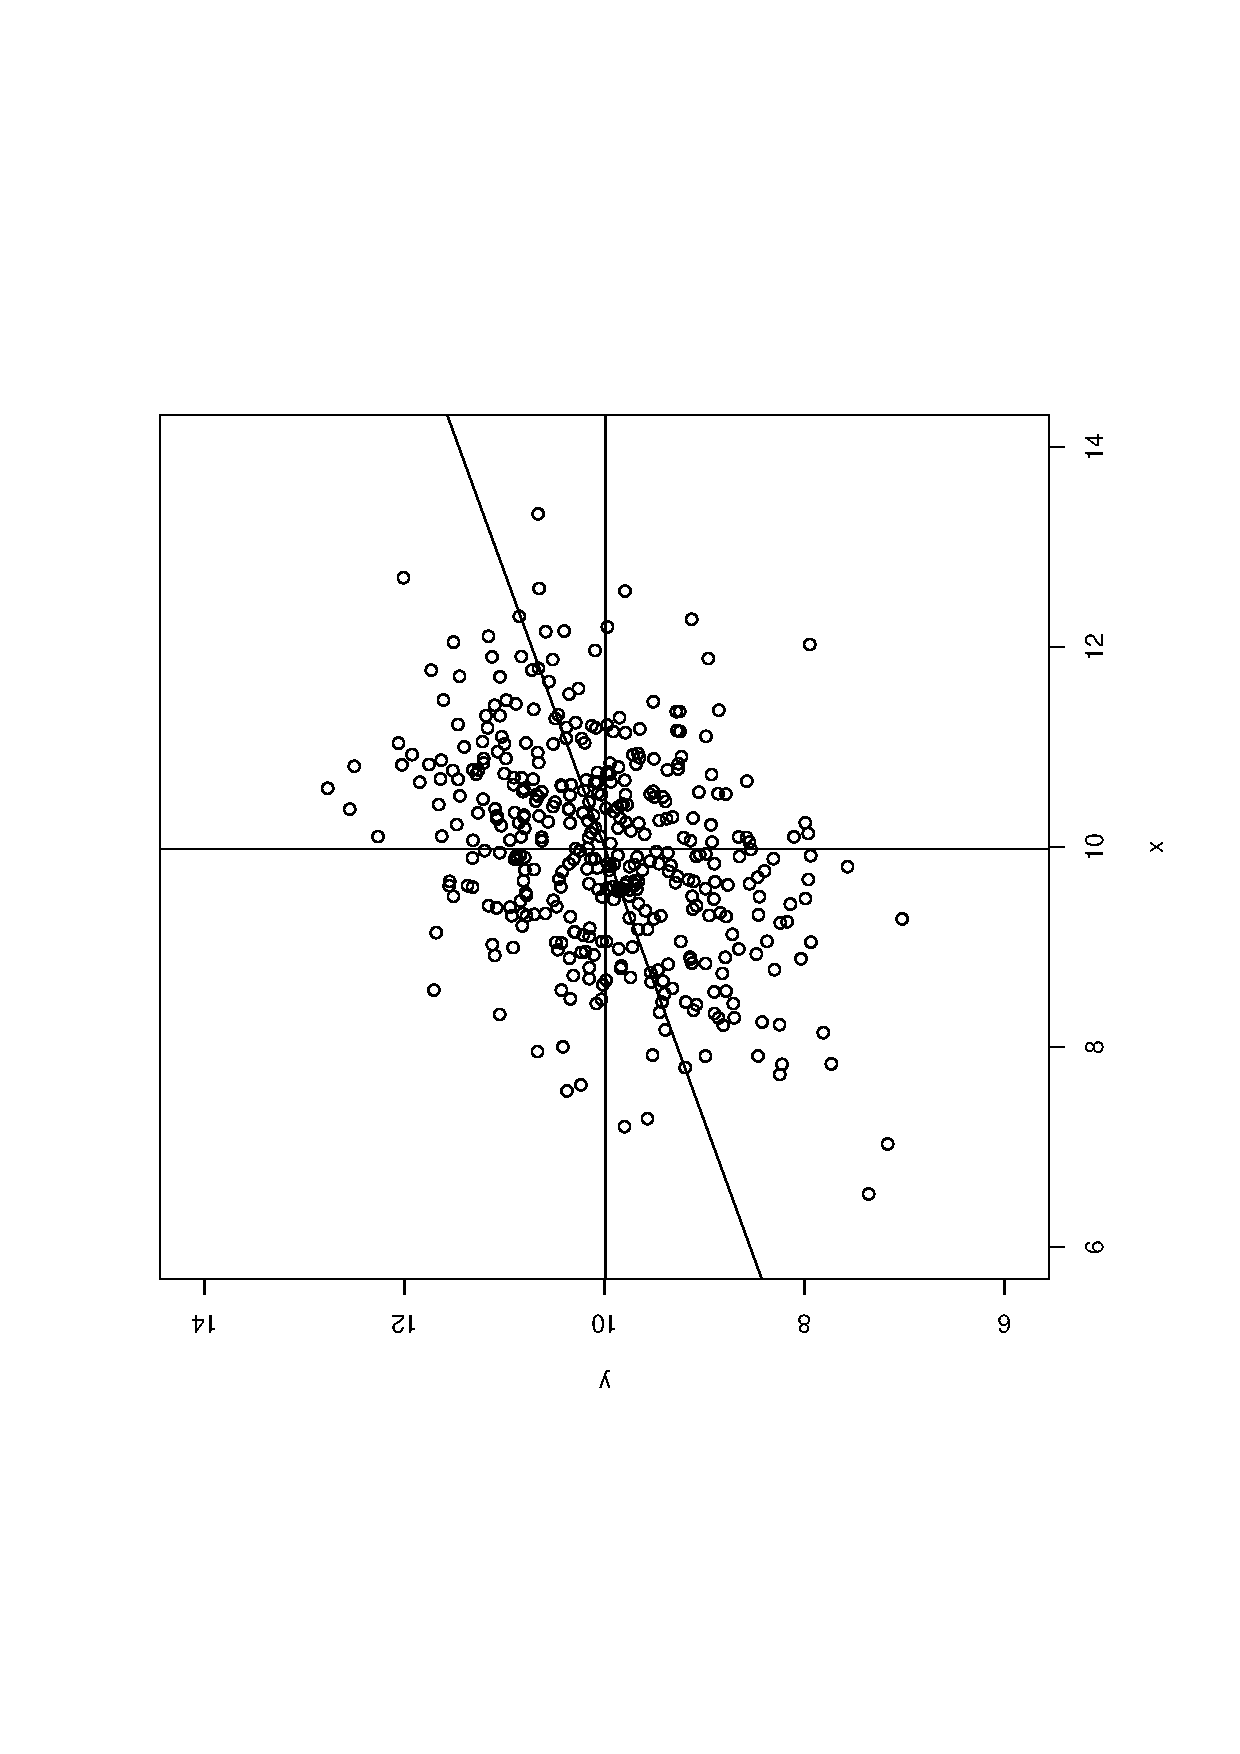
\includegraphics[height=2.6in]{opreg.idraw}}
\medskip

Expected slope is $\mathsf{~\Cov(O,P)/\Var(P) \: = \: \frac{1}{2}h^2}$.

\end{slide}

\begin{slide}[Replace]{Mean of offspring of a selected parent}
\medskip

\hspace{-0.35in}\centerline{\includegraphics[height=2.6in]{opregtrunc0.idraw}}
\medskip

Expected slope is $\mathsf{~\Cov(O,P)/\Var(P) \: = \: \frac{1}{2}h^2}$. \ 
When lots of genes of small effect add up,
get bivariate normality which implies this linear dependence.

\end{slide}

\begin{slide}[Replace]{Response to truncation selection on one parent}
\medskip

\centerline{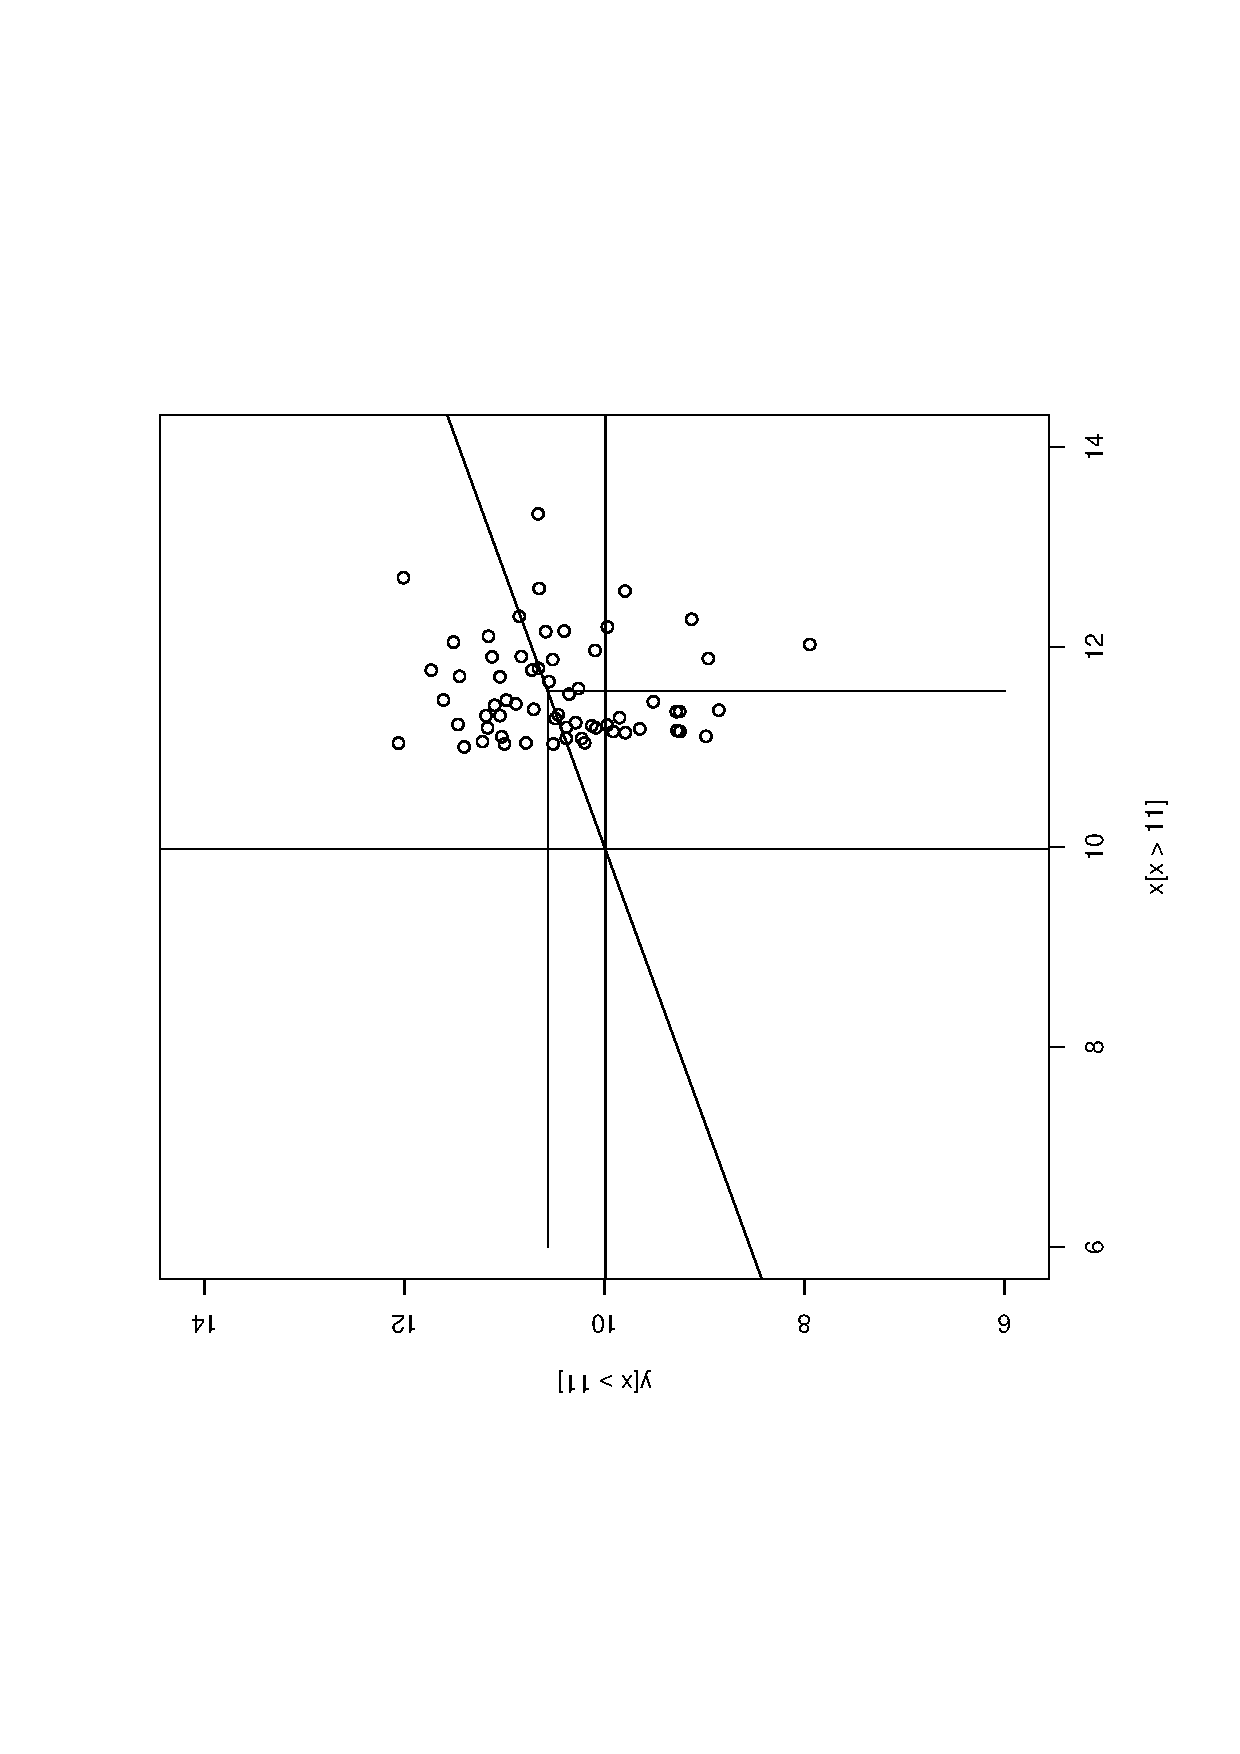
\includegraphics[height=2.6in]{opregtrunc.idraw}}
\medskip

The bivariate normality of the joint distribution implied this linear dependence.
The linearity of expectations of linear dependence guarantees this.

\end{slide}

\begin{slide}[Replace]{Response to truncation selection on both parents}
\bigskip

This response, the previous one but doubled for selection on both parents, is
the famous ``Breeder's Equation'': 
\bigskip

\hspace*{0in}\hspace{0.8in}Response = heritability $\times$ selection differential
\bigskip

(if selection is on both sexes of parent)

\end{slide}

\begin{slide}[Replace]{References on variance components and heritability}
{\parindent=-0.15in

Fisher, R. A.  1918.  On the correlation between relatives on the supposition
of Mendelian inheritance.  {\it Transactions of the Royal Society of
Edinburgh} {\bf 52:} 399-433.  \textcolor{purple}{[The great founding paper of
modern quantitative genetics. An impossible read.]}
\medskip

Lush, J. L.  1937.  {\it Animal Breeding Plans}.  Iowa State College Press,
Ames, Iowa.  \textcolor{purple}{[The book that brought quantitative genetics
to animal breeding]}  (Also available online in its 1943 edition at
\textcolor{brightred}{\url{http://archive.org/details/animalbreedingpl032391mbp}} )
\medskip

Falconer, D. S. and T. F. C. MacKay.  1996. {\it An Introduction to Quantitative
Genetics}.  4th Edition.  Benjamin-Cummings, San Francisco.
\textcolor{purple}{[Falconer's classic 1960 textbook, updated in recent
editions by Trudy MacKay]}
\medskip

Lynch, M. and B. Walsh.  1998.  {\it Genetics and Analysis of Quantitative
Traits}.  Sinauer Associates, Sunderland, Massachusetts. \textcolor{purple}{[A
recent and more intensive and comprehensive text]}
\medskip

}
\end{slide}

\begin{slide}[Replace]{References on variance components and heritability}
{\parindent=-0.15in

Chapter drafts of Lynch and Walsh's forthcoming two-volume ``Volume 2'' are free online
at Bruce Walsh's web site:
\hspace*{0in}\hspace{-0.15in}\textcolor{brightred}{\tiny \url{http://nitro.biosci.arizona.edu/zbook/NewVolume_2/newvol2.html}}

The first part of "Volume 2" is expected to be published by Sinauer Associates,
maybe soon.
\medskip

Felsenstein, J.  2015.  {\it Theoretical Evolutionary Genetics}. Available
as a free download from the  Department of Genome Sciences, University of
Washington, Seattle at
\textcolor{brightred}{\url{http://evolution.gs.washington.edu/pgbook/pgbook.html}}
\textcolor{purple}{[My population genetics theory class text; chapter IX
covers quantitative genetics theory]}
}

\end{slide}
}

\end{document}
